\chapter{Histograms}
\label{app:hist}

In the following pages we include the histograms of the distributions of the log-returns for each of the assets in our dataset. We superimpose to the histograms the graphs of the density functions obtained using the three models of Merton, Heston and Bates with the calibrated parameters shown in Tables \ref{tab:merton_params}, \ref{tab:heston_params} and \ref{tab:bates_params}.

We can see that given our results from the calibration, Heston and Bates better approximate the empirical distribution of the returns in all cases.

\begin{figure}
	\small
	\centering
	\begin{subfigure}{0.44\textwidth}
		\centering
		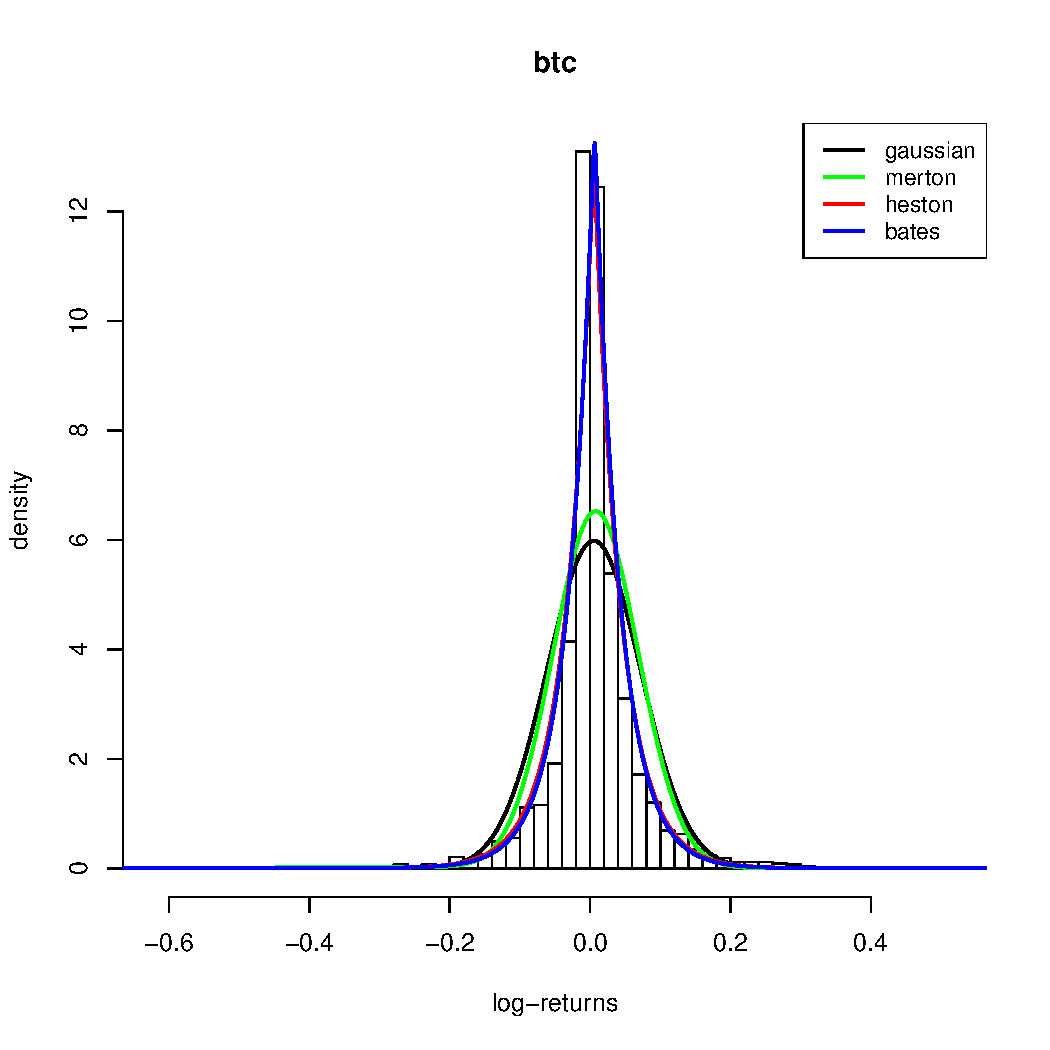
\includegraphics[width=\linewidth]{Images/hist_btc.pdf}
		\caption{Bitcoin}
	\end{subfigure}
	\begin{subfigure}{0.44\textwidth}
		\centering
		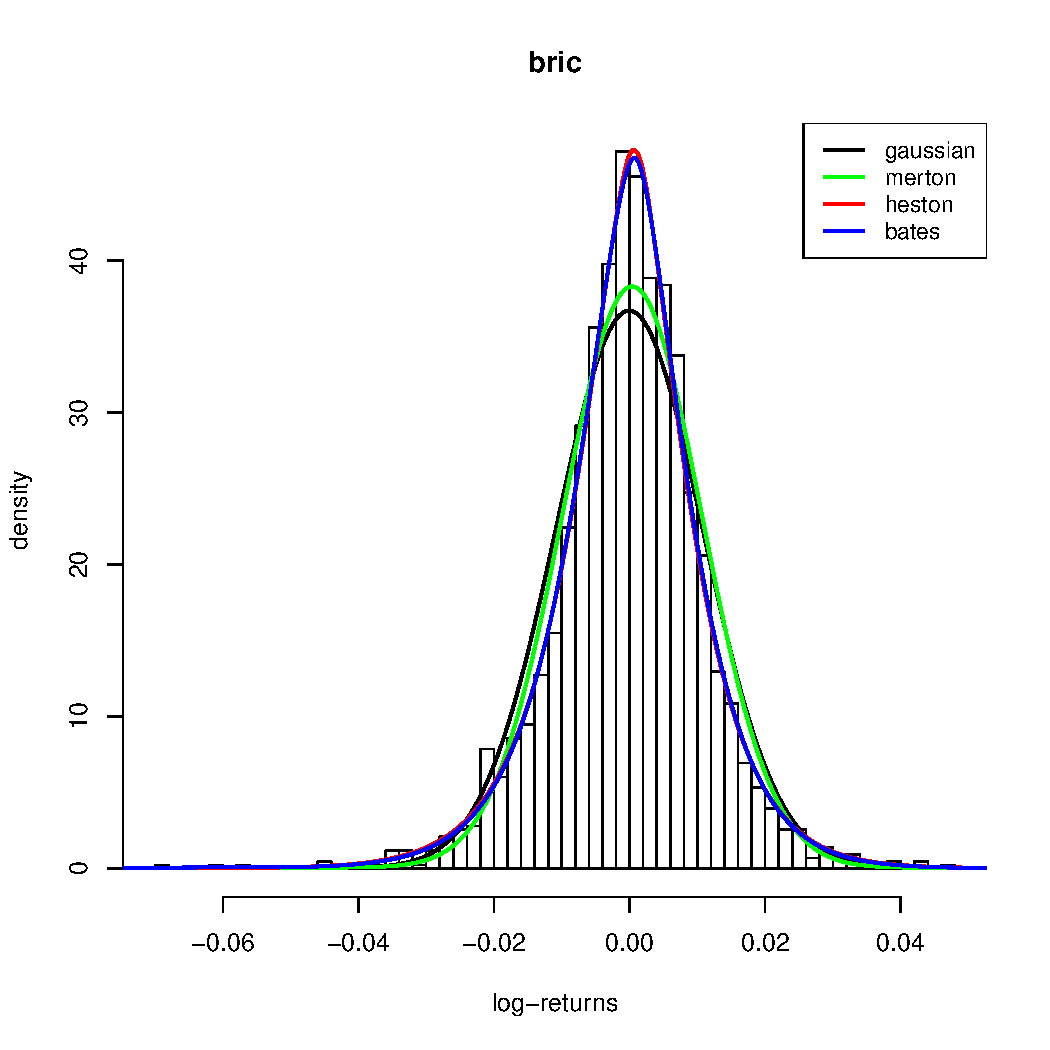
\includegraphics[width=\linewidth]{Images/hist_bric.pdf}
		\caption{Bric index}
	\end{subfigure}
	\\
	\begin{subfigure}{0.44\textwidth}
		\centering
		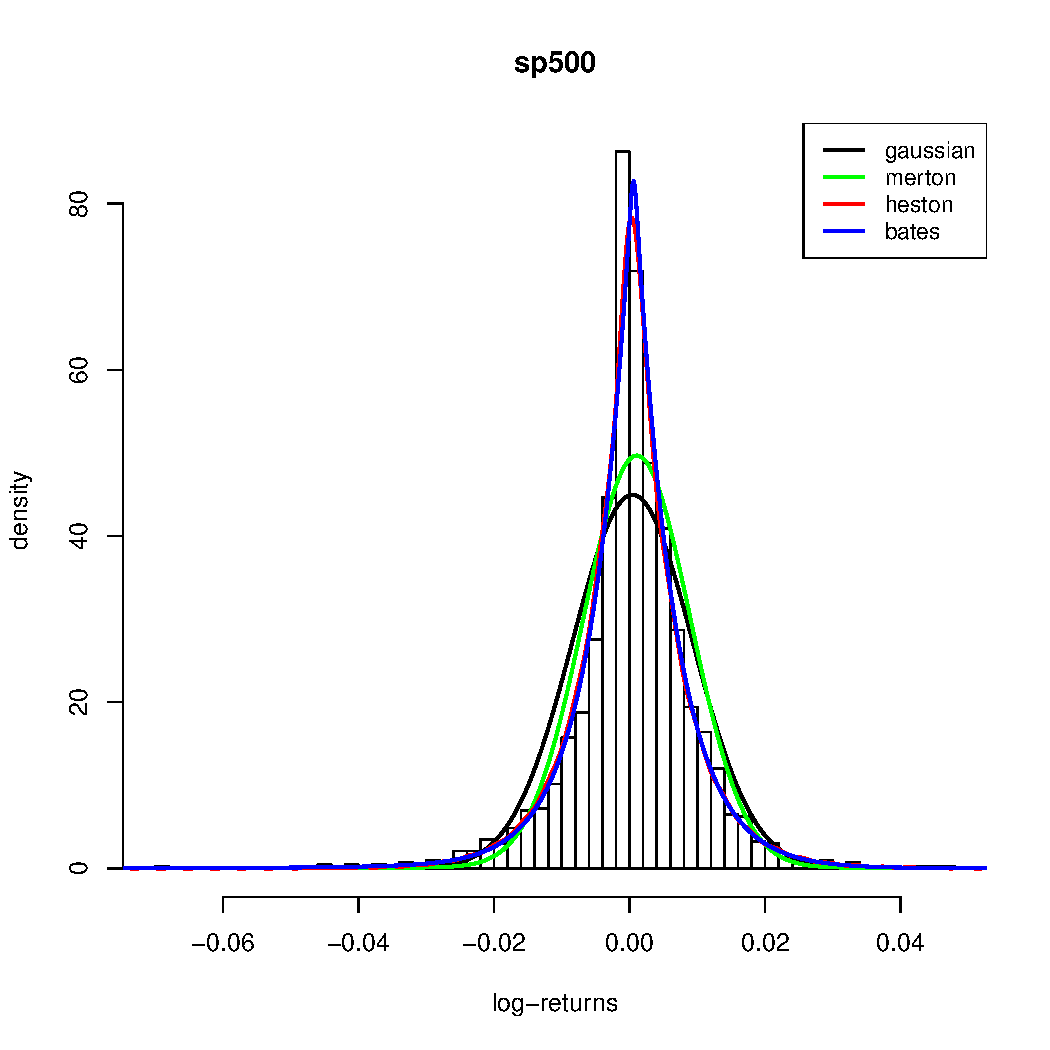
\includegraphics[width=\linewidth]{Images/hist_sp500.pdf}
		\caption{S\&P500}
	\end{subfigure}
	\begin{subfigure}{0.44\textwidth}
		\centering
		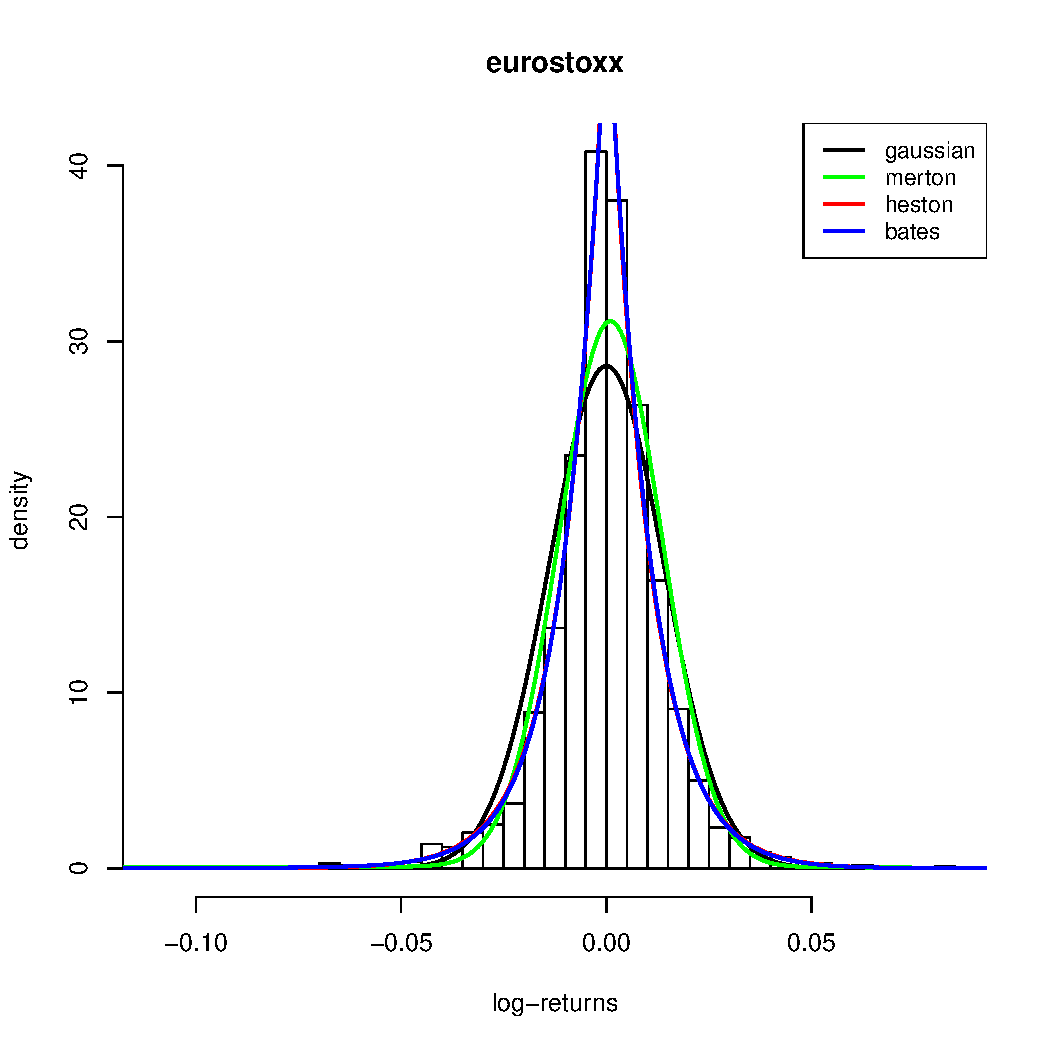
\includegraphics[width=\linewidth]{Images/hist_eurostoxx.pdf}
		\caption{Eurostoxx50}
	\end{subfigure}
	\caption[Histrogram and densities of the results (1/3)]{Histogram of the log-returns and pdf for the three models we calibrated and the Gaussian line as reference.[1/3]}
	\label{fig:hist_1}
	
\end{figure}





\begin{figure}
	\small
	\centering
	\begin{subfigure}{0.44\textwidth}
		\centering
		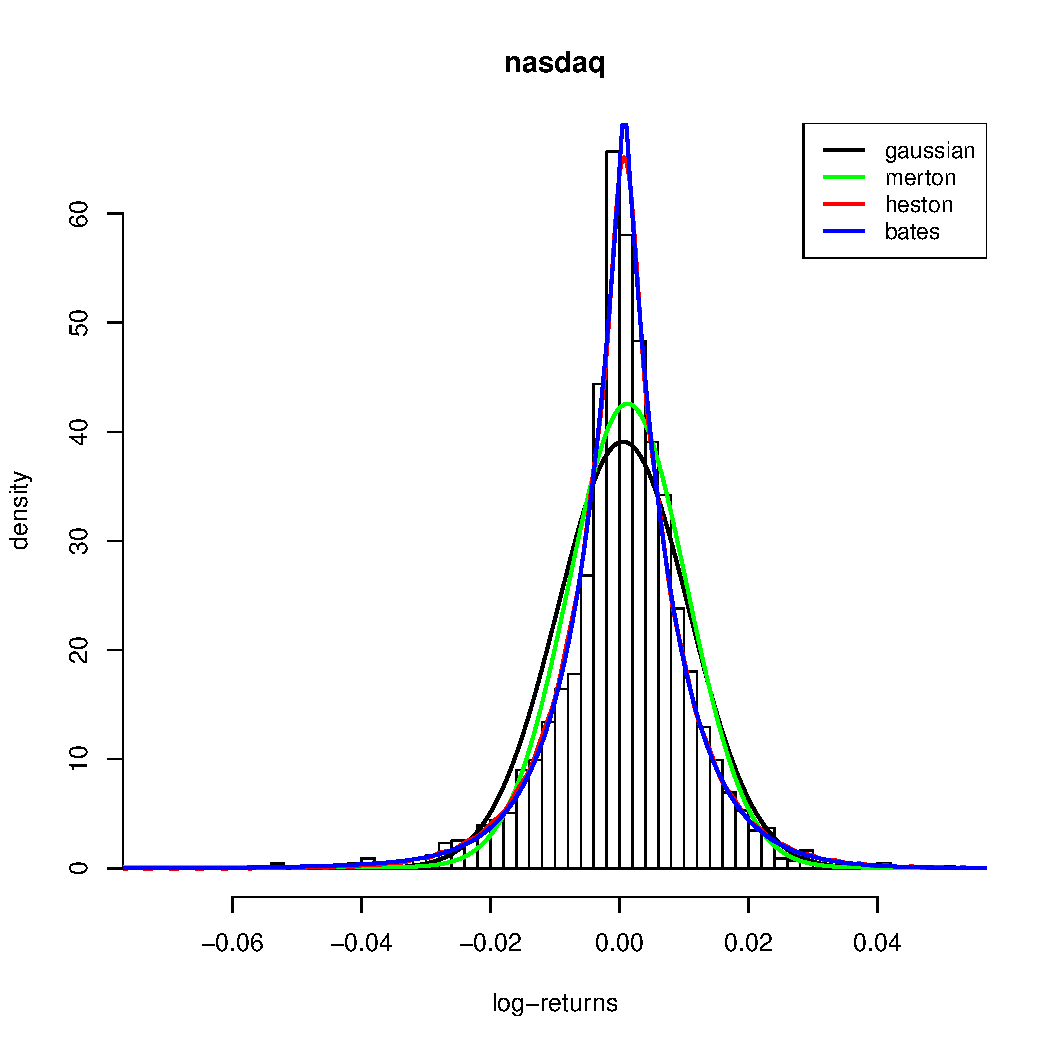
\includegraphics[width=\linewidth]{Images/hist_nasdaq.pdf}
		\caption{Nasdaq}
	\end{subfigure}
	\begin{subfigure}{0.44\textwidth}
		\centering
		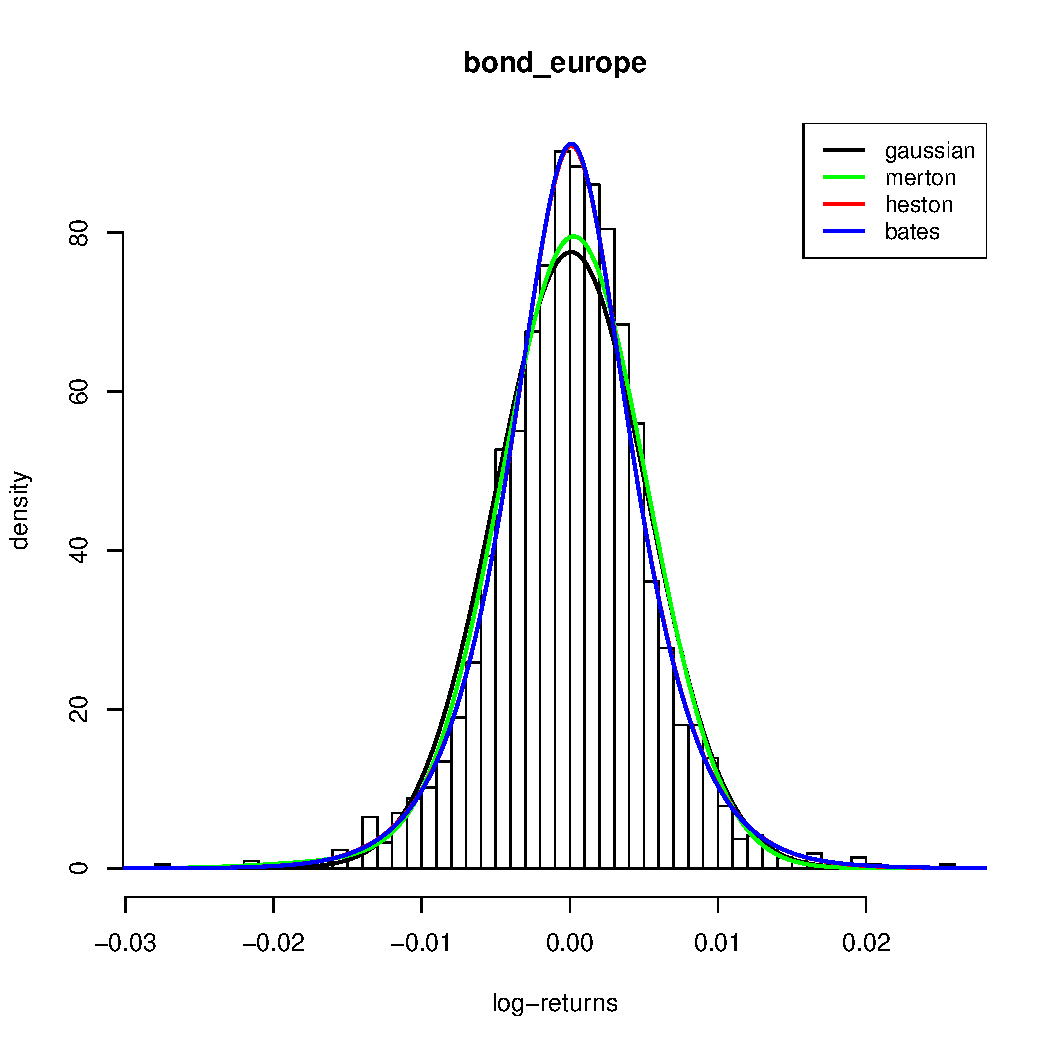
\includegraphics[width=\linewidth]{Images/hist_bond_europe.pdf}
		\caption{Bond Europe}
	\end{subfigure}

\begin{subfigure}{0.44\textwidth}
	\centering
	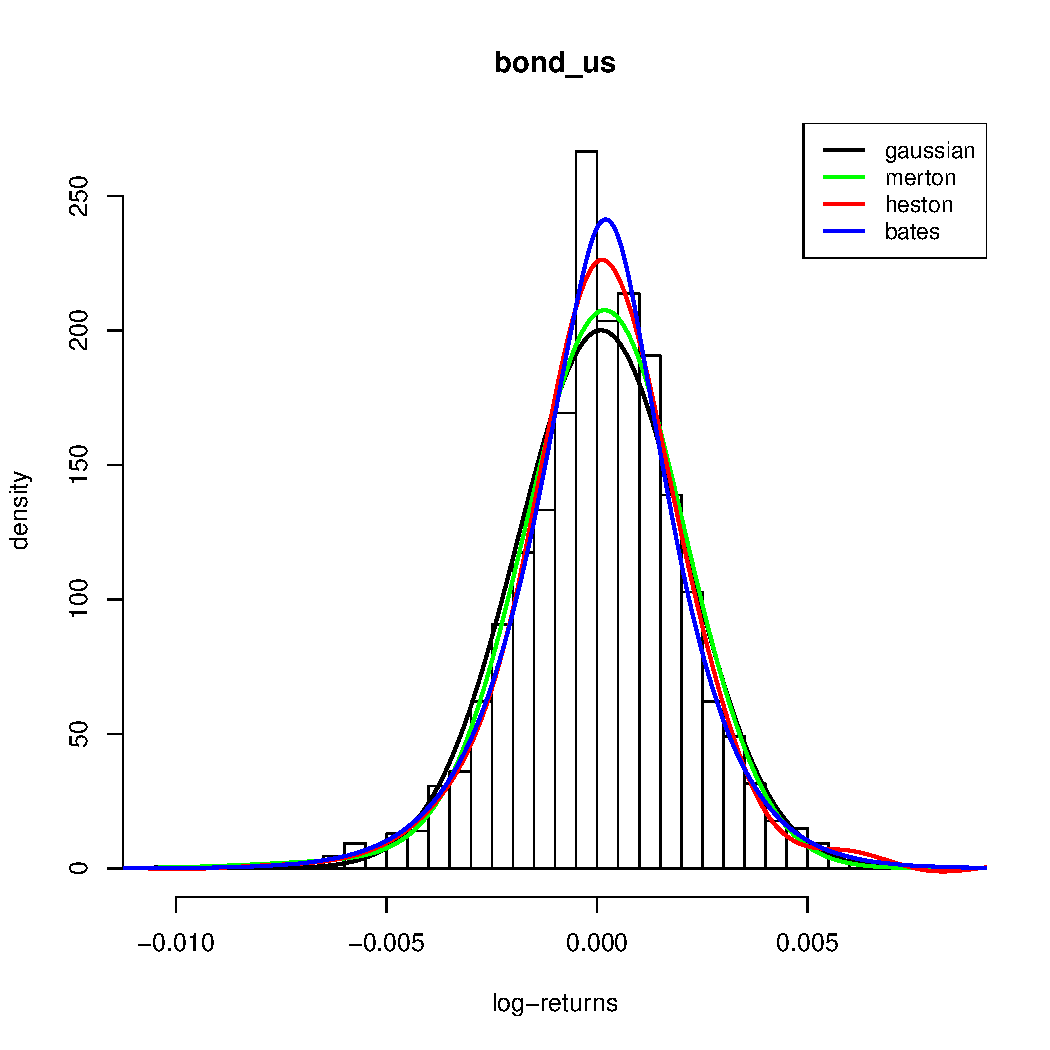
\includegraphics[width=\linewidth]{Images/hist_bond_us.pdf}
	\caption{Bond US}
\end{subfigure}
\begin{subfigure}{0.44\textwidth}
	\centering
	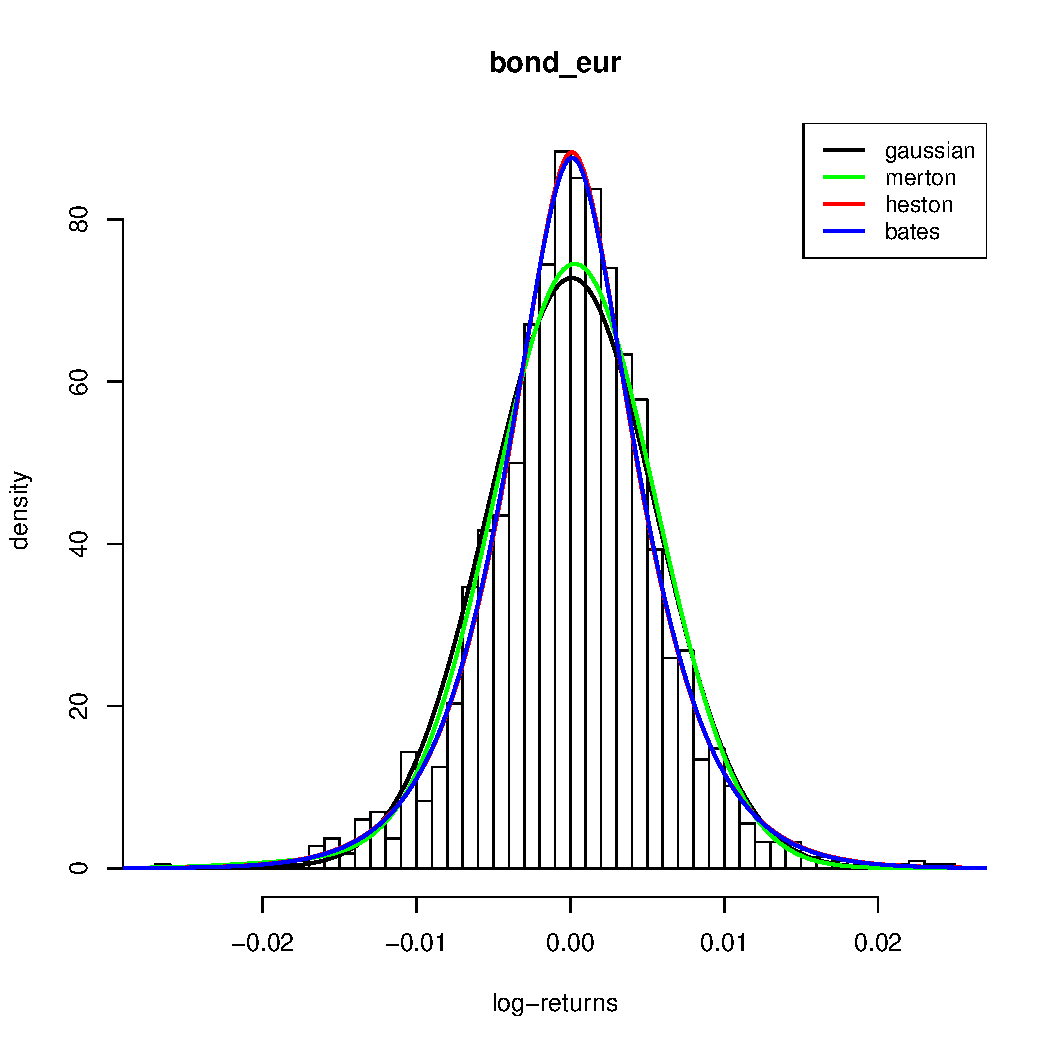
\includegraphics[width=\linewidth]{Images/hist_bond_eur.pdf}
	\caption{Bond EUR}
\end{subfigure}

\begin{subfigure}{0.44\textwidth}
	\centering
	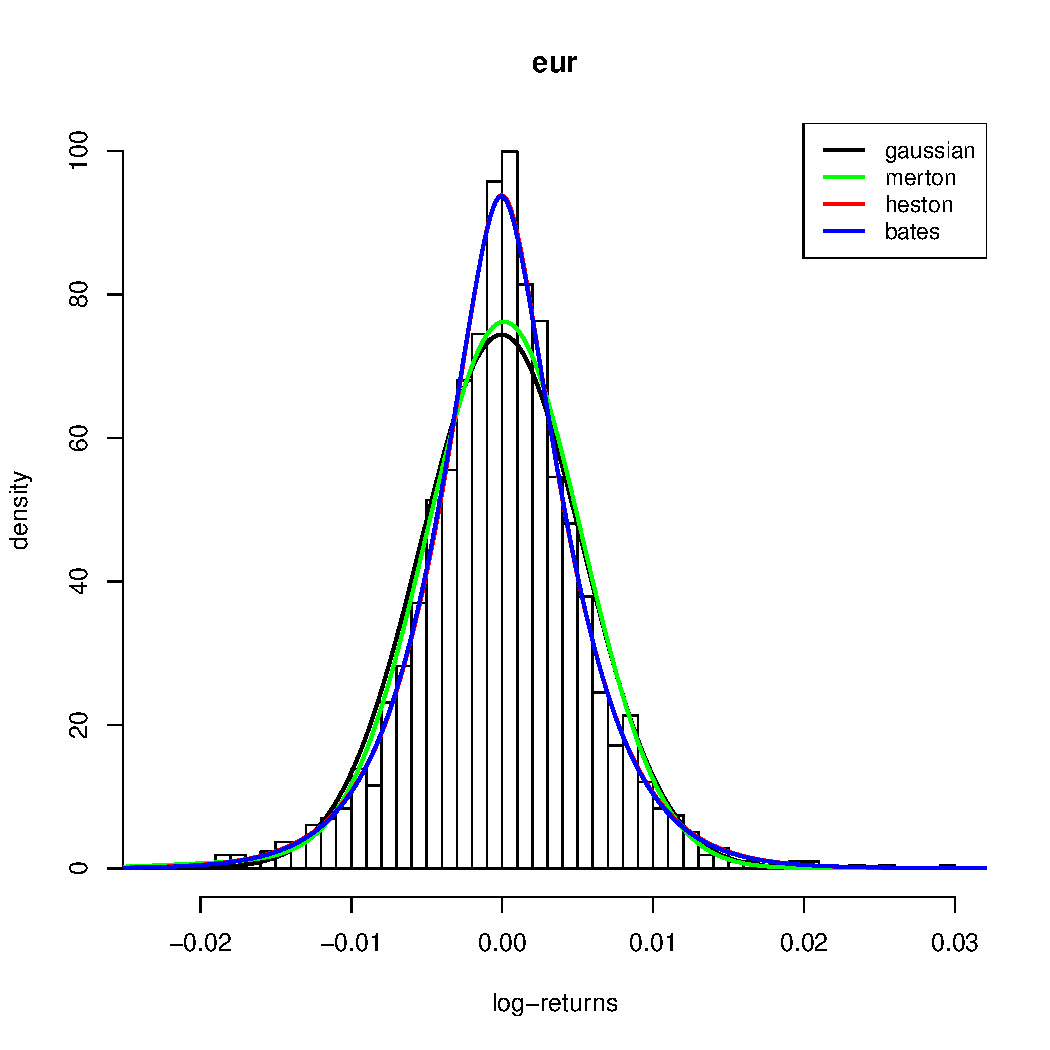
\includegraphics[width=\linewidth]{Images/hist_eur.pdf}
	\caption{EUR/USD}
\end{subfigure}
\begin{subfigure}{0.44\textwidth}
	\centering
	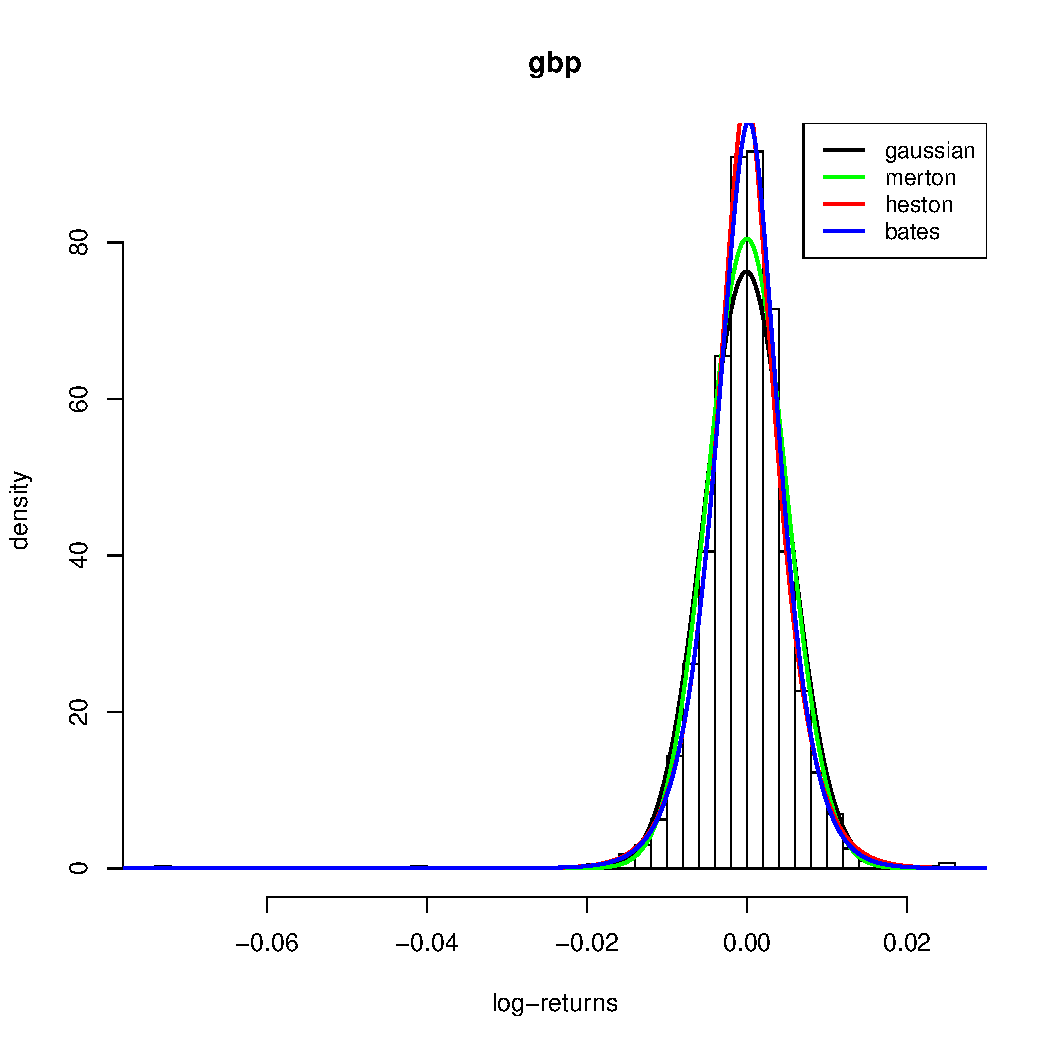
\includegraphics[width=\linewidth]{Images/hist_gbp.pdf}
	\caption{GBP/USD}
\end{subfigure}

\caption[Histrogram and densities of the results (2/3)]{Histogram of the log-returns and pdf for the three models we calibrated and the Gaussian line as reference.[2/3]}
\label{fig:hist_2}
\end{figure}


\begin{figure}
	\small
	\centering
	\begin{subfigure}{0.44\textwidth}
		\centering
		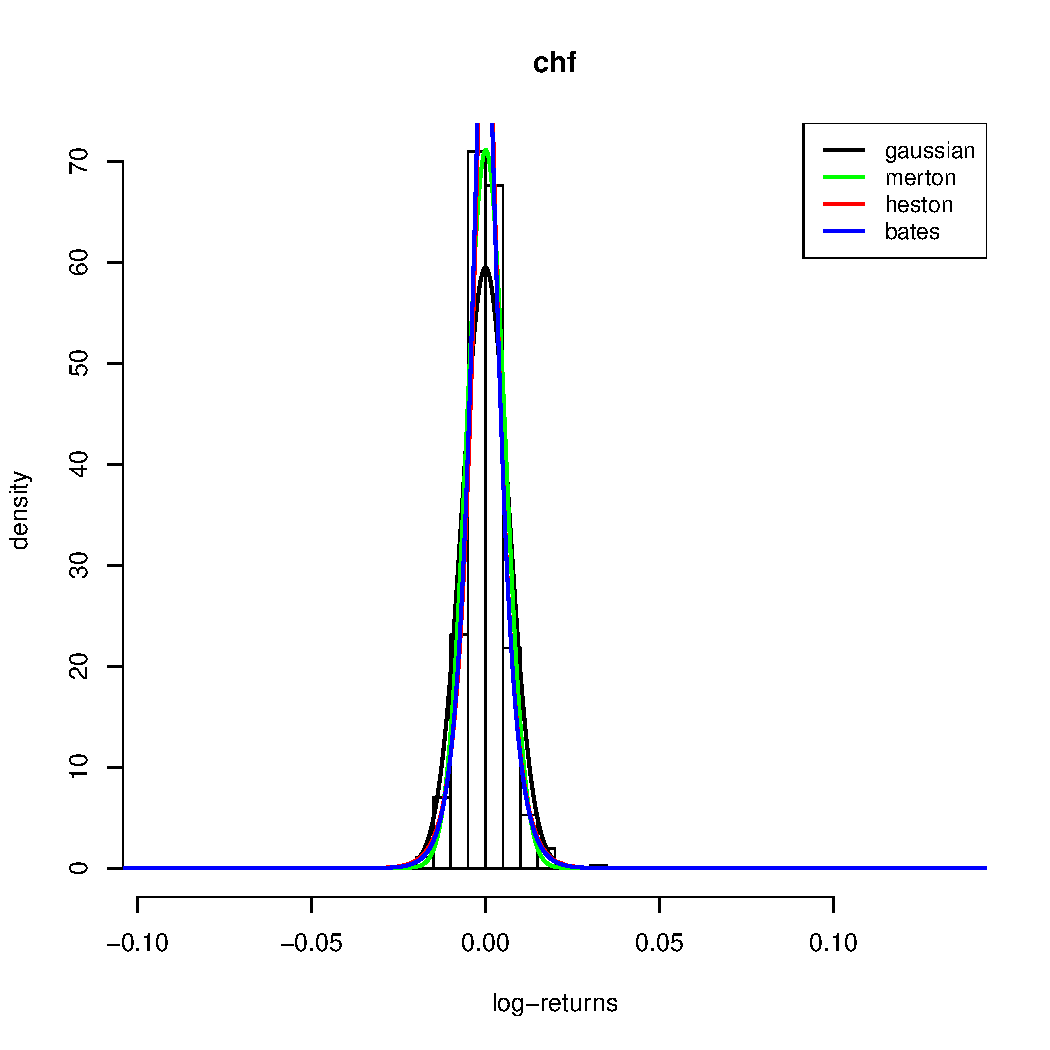
\includegraphics[width=\linewidth]{Images/hist_chf.pdf}
		\caption{CHF/USD}
	\end{subfigure}
	\begin{subfigure}{0.44\textwidth}
		\centering
		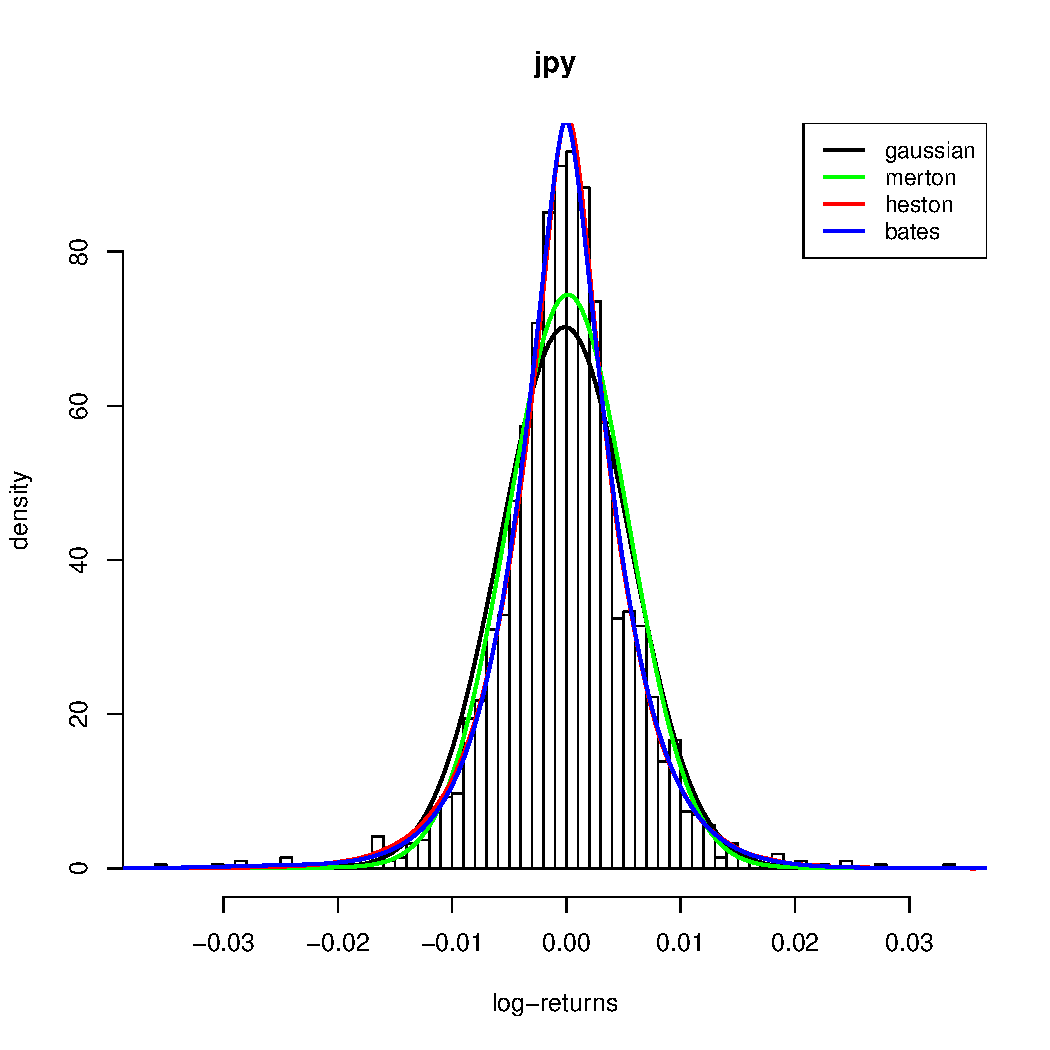
\includegraphics[width=\linewidth]{Images/hist_jpy.pdf}
		\caption{JPY/USD}
	\end{subfigure}
	
	\begin{subfigure}{0.44\textwidth}
		\centering
		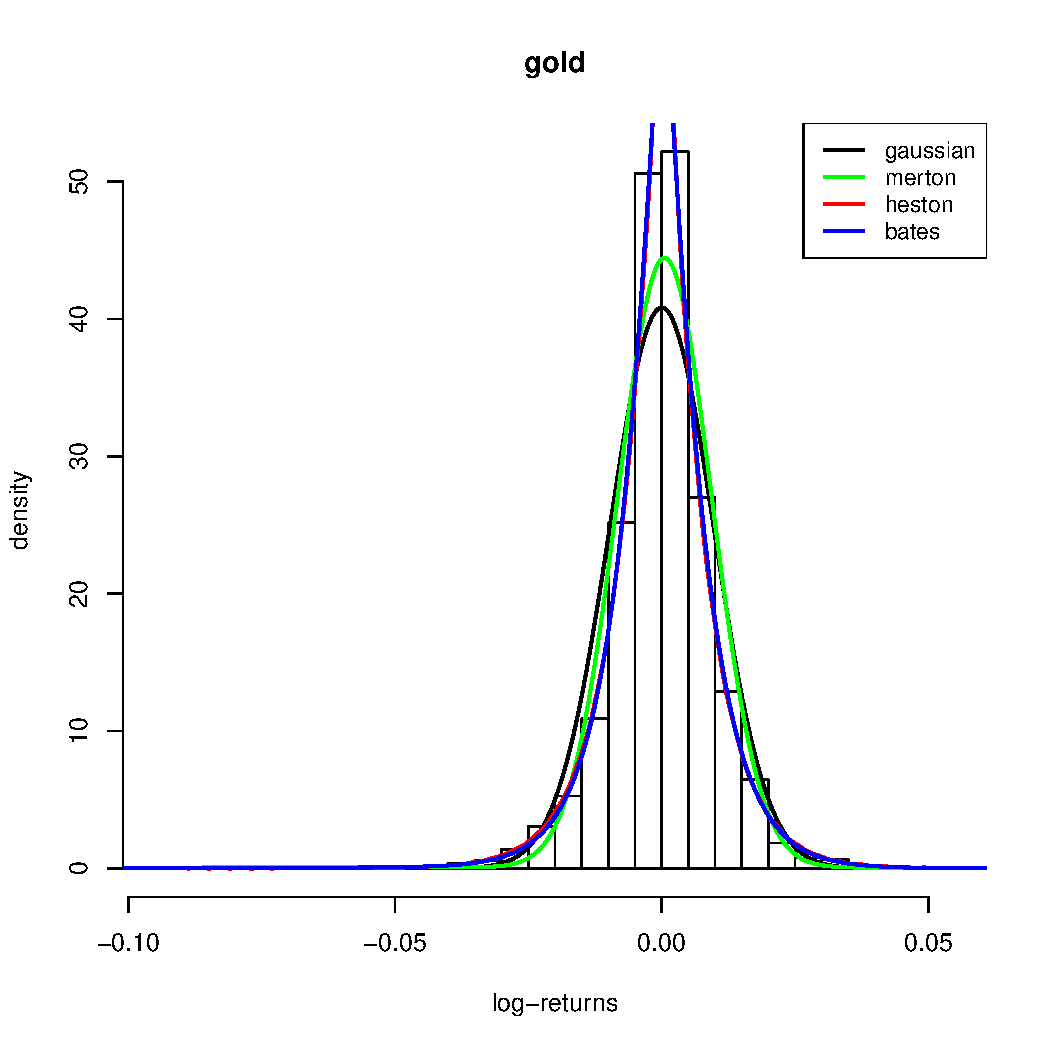
\includegraphics[width=\linewidth]{Images/hist_gold.pdf}
		\caption{Gold}
	\end{subfigure}
	\begin{subfigure}{0.44\textwidth}
		\centering
		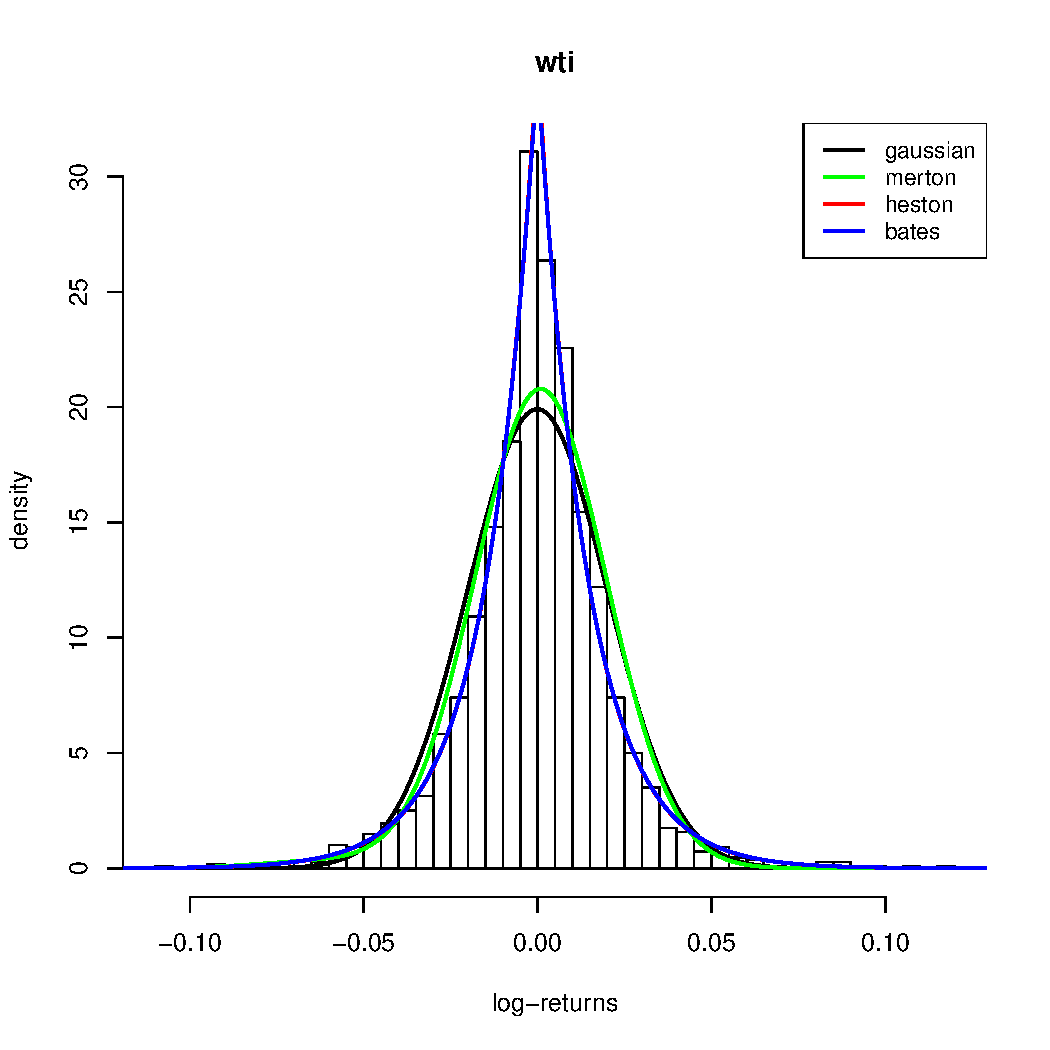
\includegraphics[width=\linewidth]{Images/hist_wti.pdf}
		\caption{Wti oil}
	\end{subfigure}
	
	\begin{subfigure}{0.44\textwidth}
		\centering
		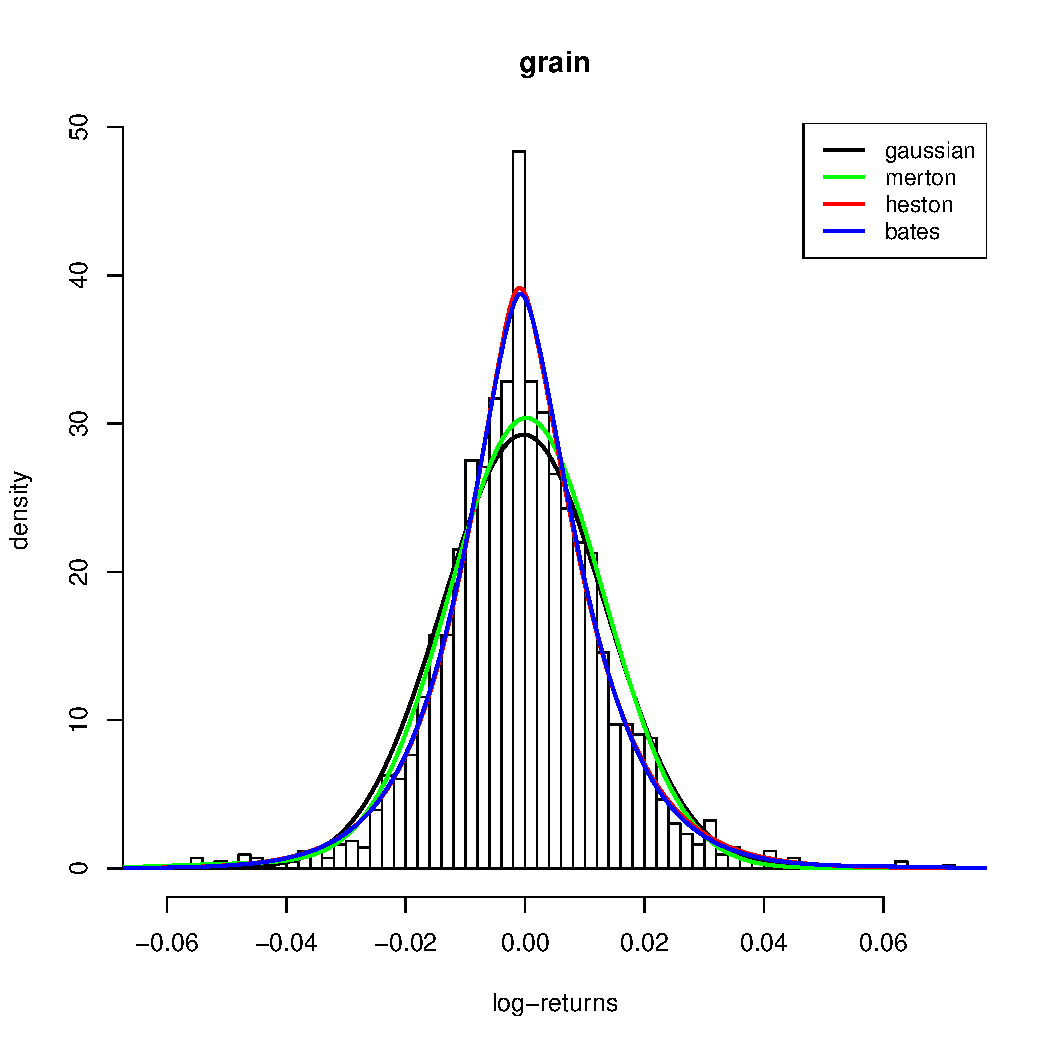
\includegraphics[width=\linewidth]{Images/hist_grain.pdf}
		\caption{Grain}
	\end{subfigure}
	\begin{subfigure}{0.44\textwidth}
		\centering
		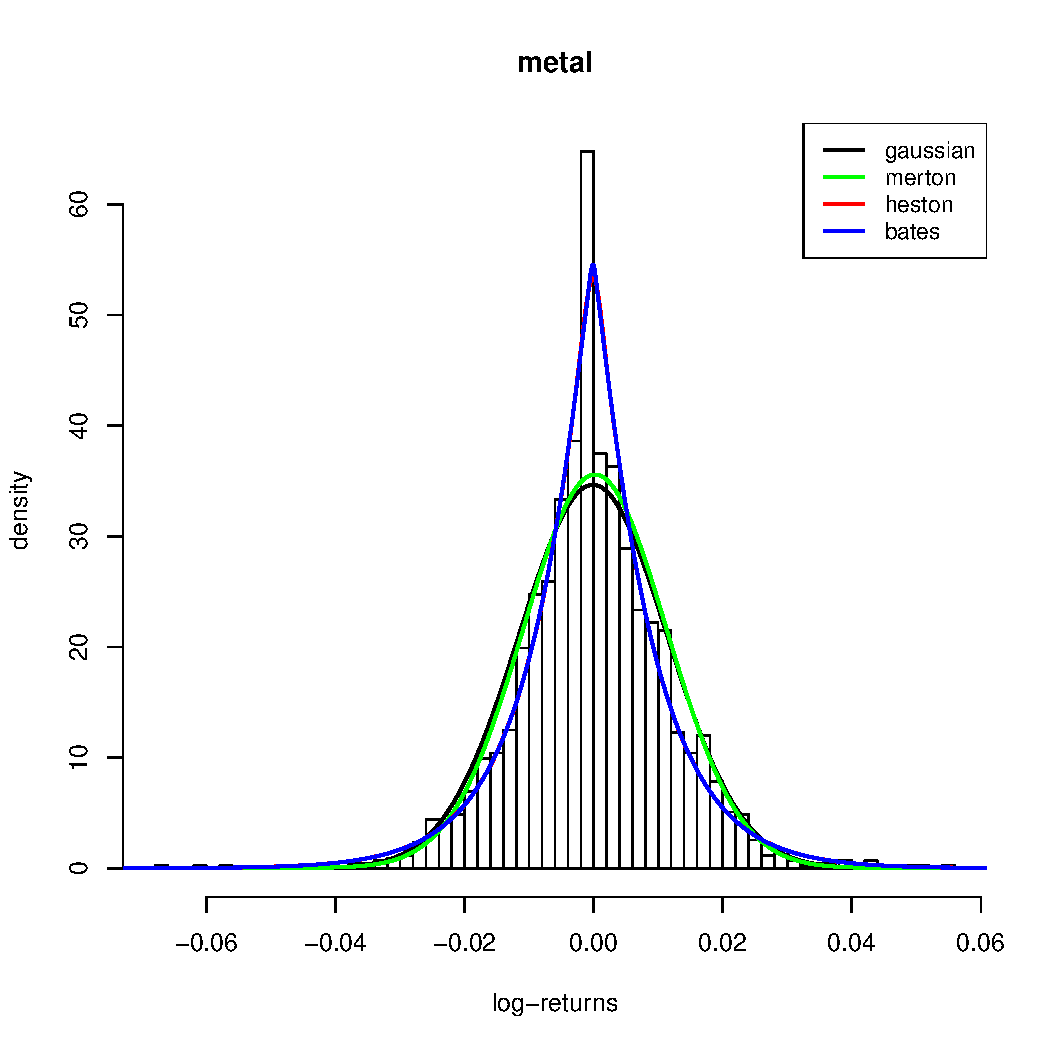
\includegraphics[width=\linewidth]{Images/hist_metal.pdf}
		\caption{Metals}
	\end{subfigure}
	
	\caption[Histrogram and densities of the results (3/3)]{Histogram of the log-returns and pdf for the three models we calibrated and the Gaussian line as reference. [3/3]}
	\label{fig:hist_3}
\end{figure}

%\\
%\begin{subfigure}{0.44\textwidth}
%	\centering
%	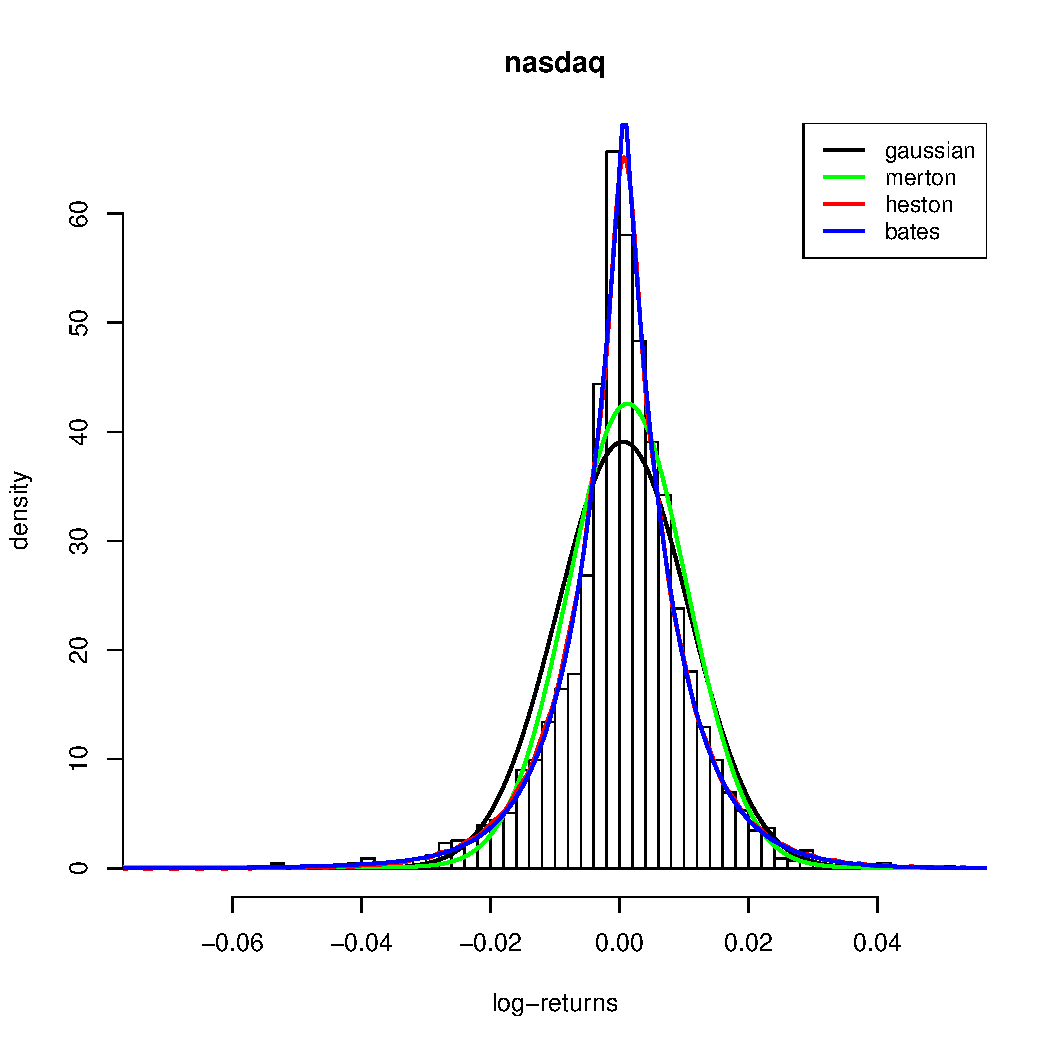
\includegraphics[width=\linewidth]{Images/hist_nasdaq.pdf}
%	\caption{text}
%\end{subfigure}
%\begin{subfigure}{0.44\textwidth}
%	\centering
%	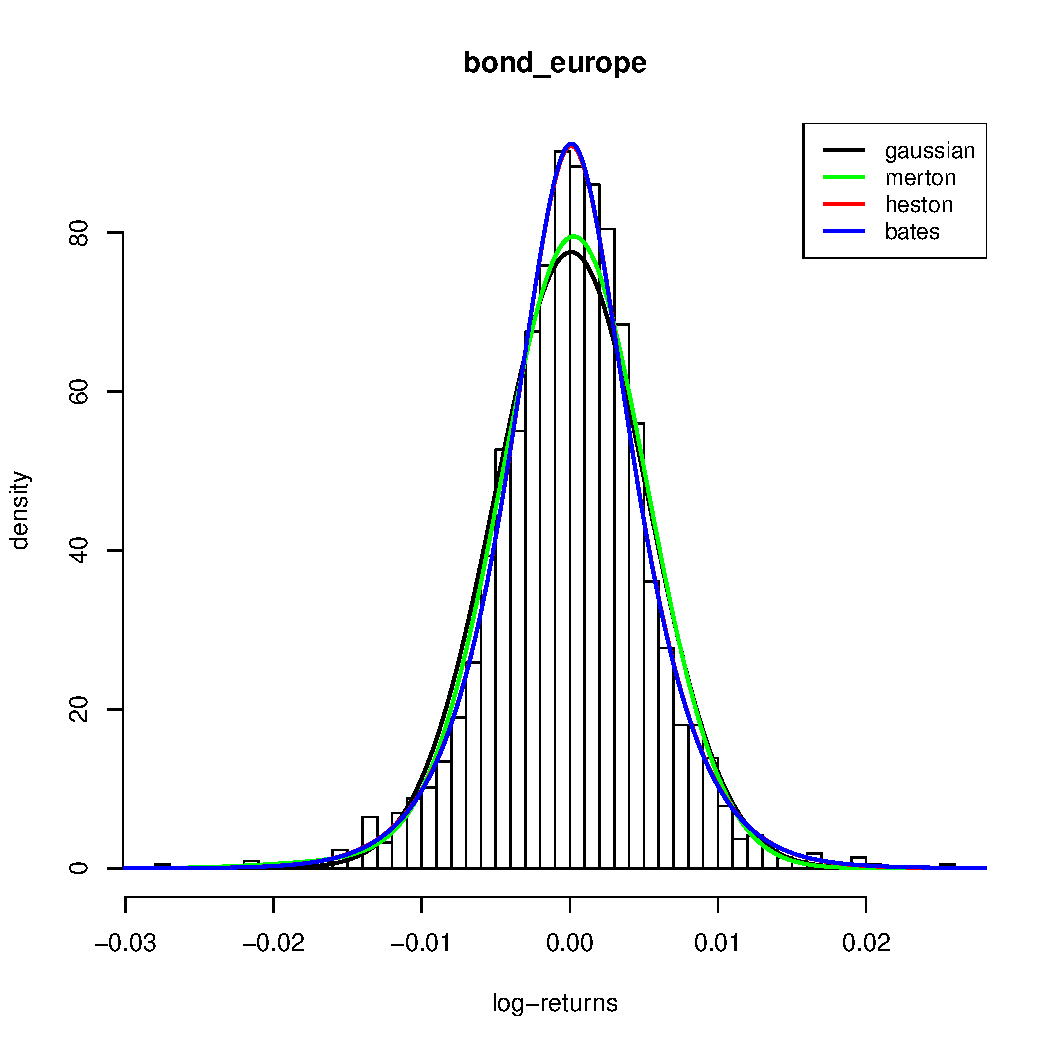
\includegraphics[width=\linewidth]{Images/hist_bond_europe.pdf}
%	\caption{text}
%\end{subfigure}

%	\hspace{0mm}
%\subfloat[Nasdaq]{   
%	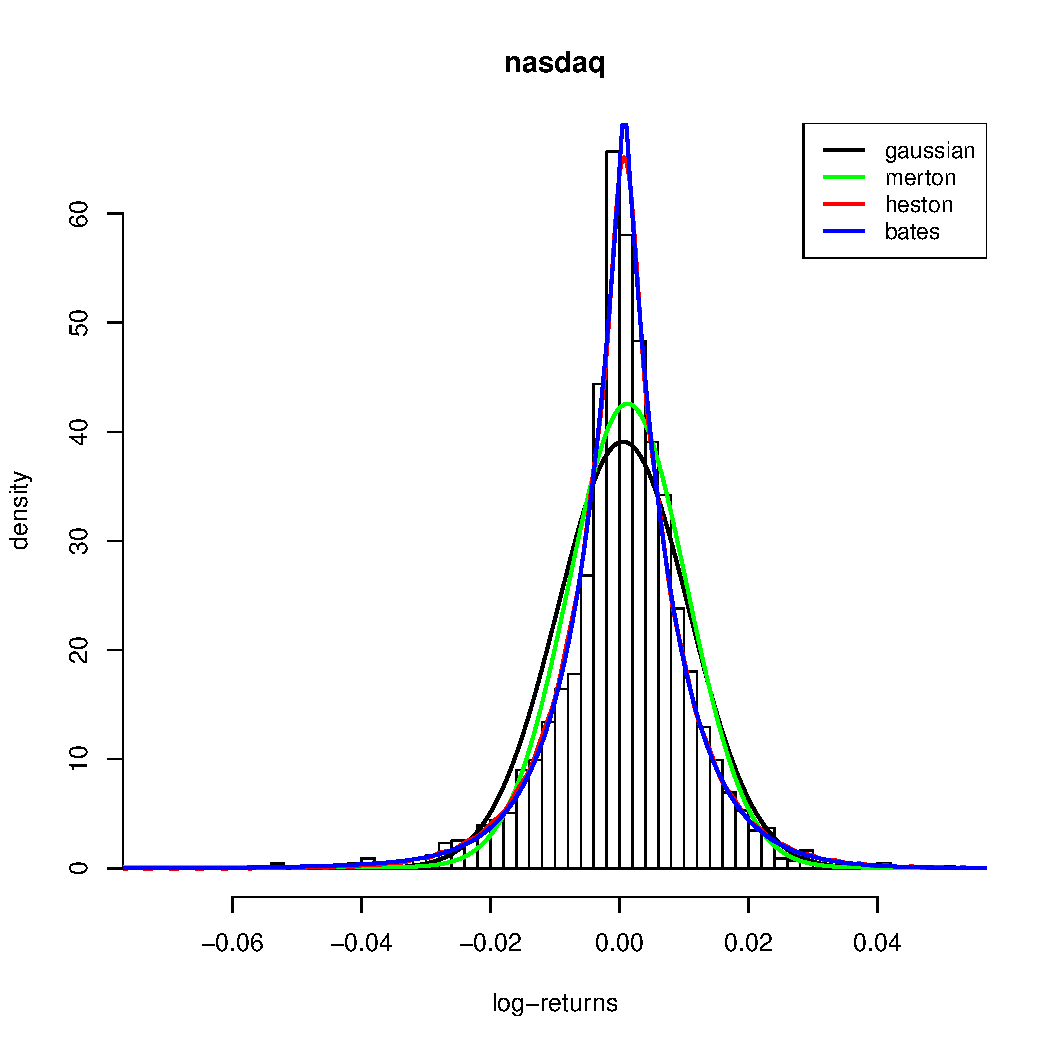
\includegraphics[height=0.3\textheight]{Images/hist_nasdaq.pdf}
%}
%\subfloat[Bond Europe]{
%	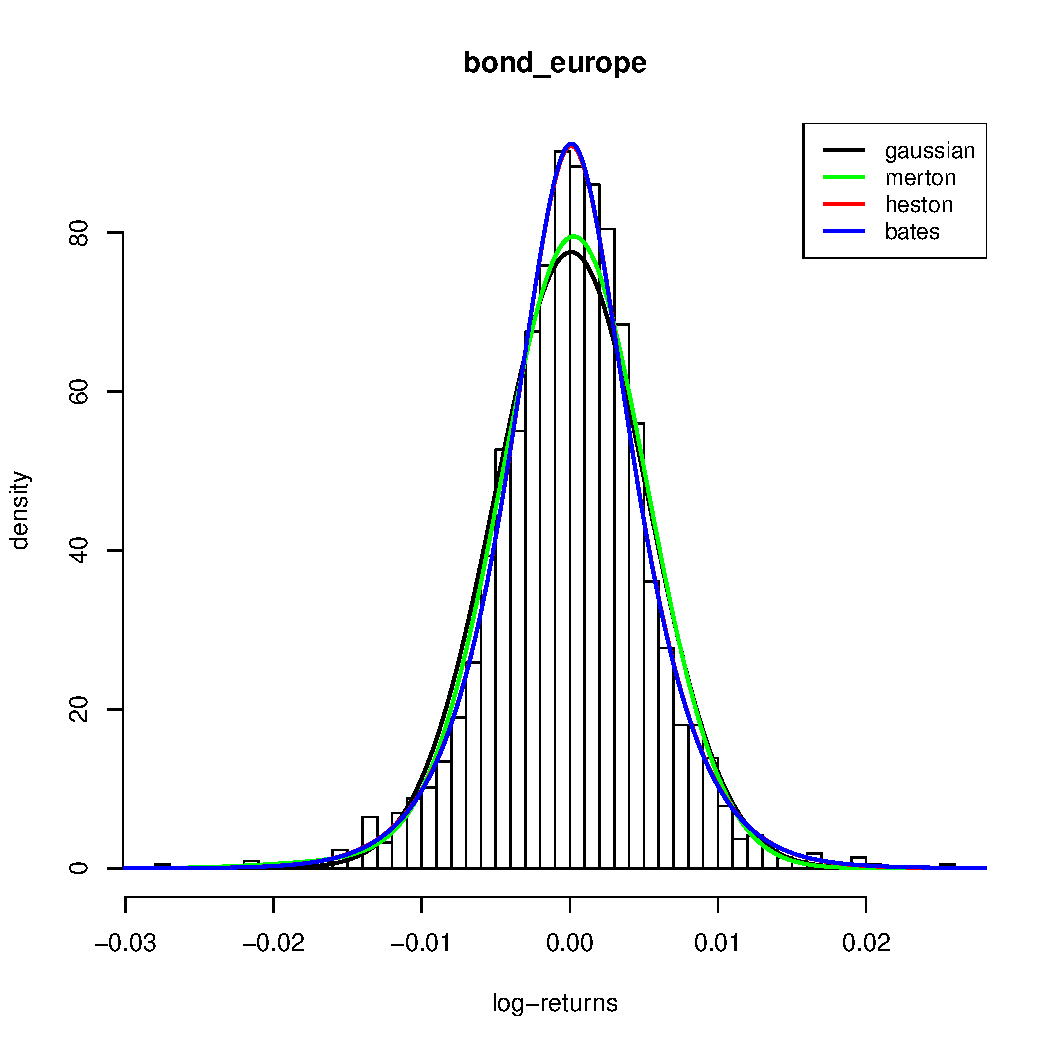
\includegraphics[height=0.3\textheight]{Images/hist_bond_europe.pdf}
%}

%	\hspace{0mm}
%\subfloat[Bond US]{   
%	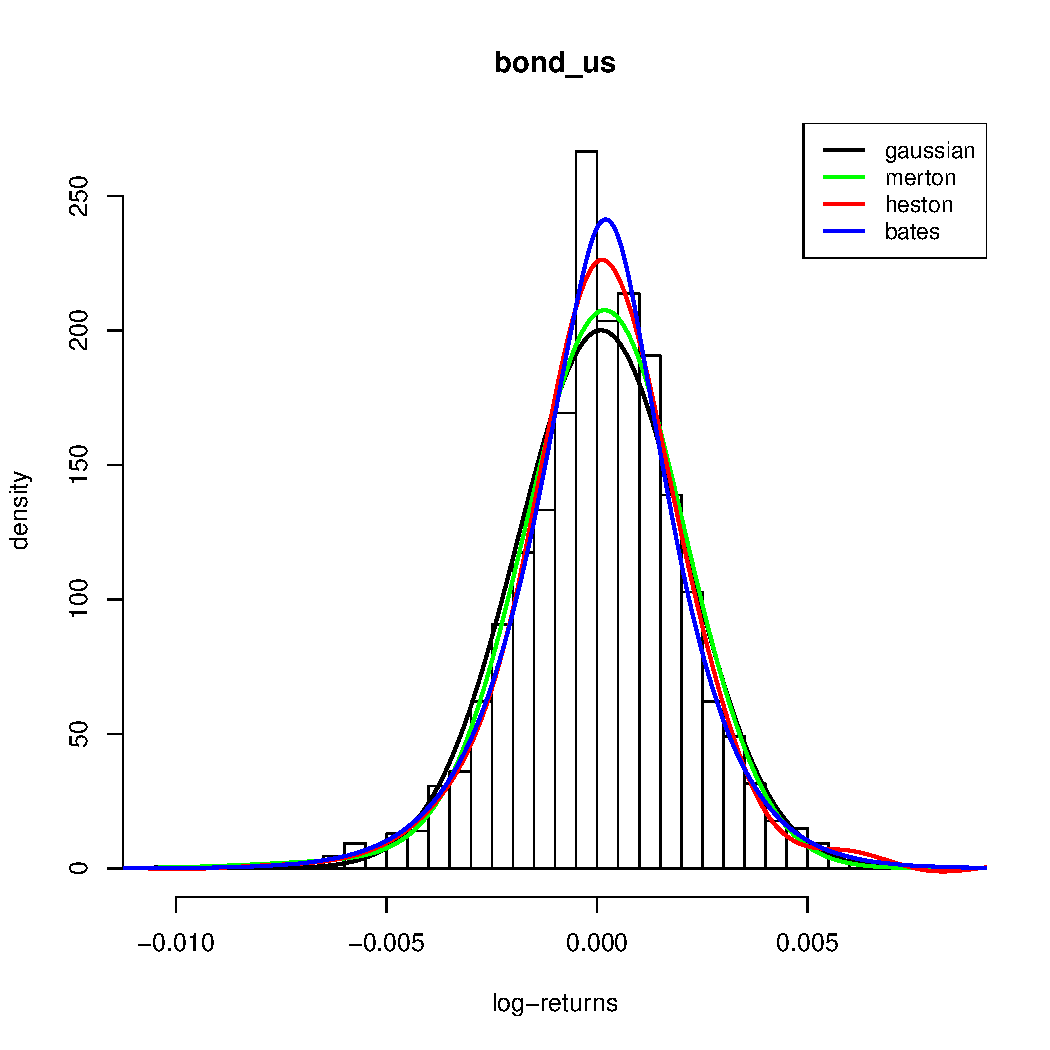
\includegraphics[height=0.3\textheight]{Images/hist_bond_us.pdf}
%}
%\subfloat[Bond EUR]{
%	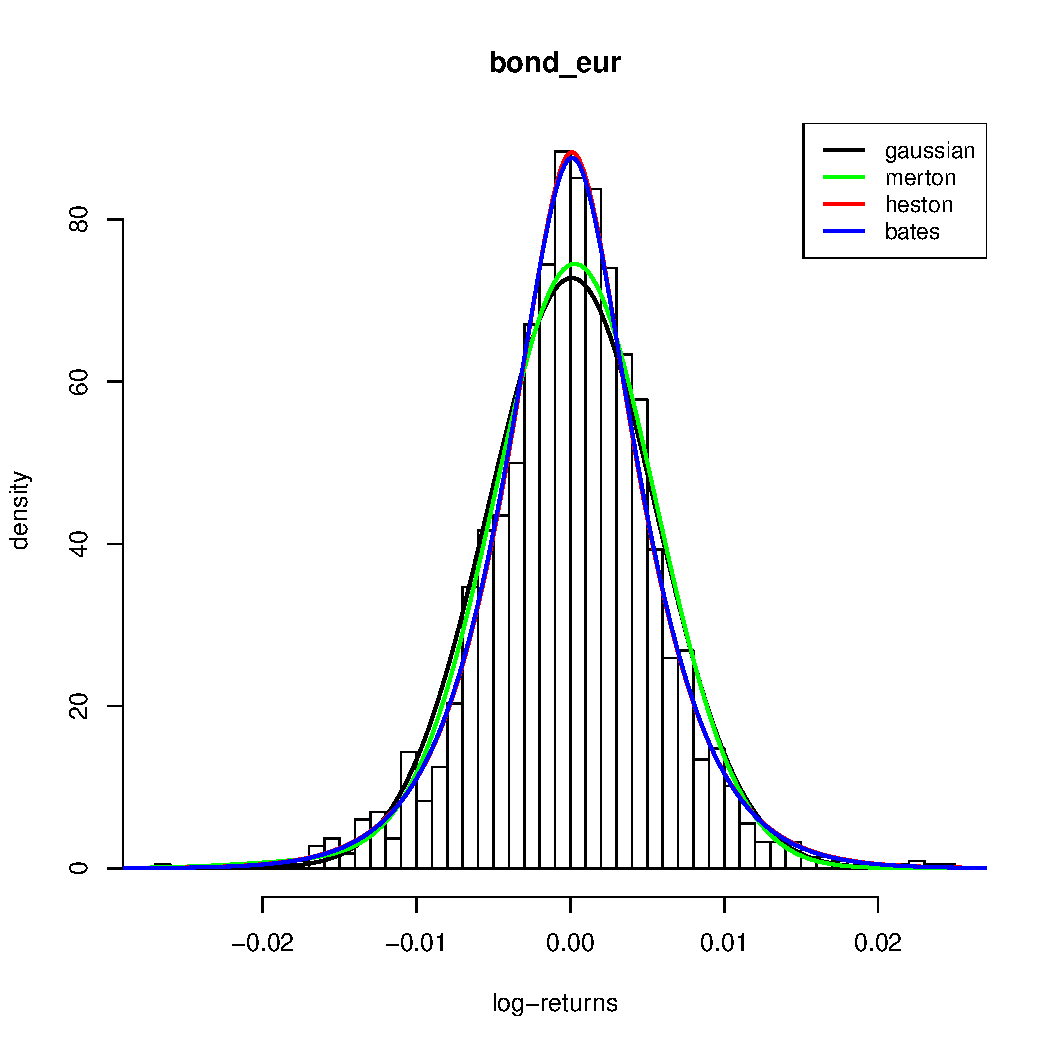
\includegraphics[height=0.3\textheight]{Images/hist_bond_eur.pdf}
%}